\textit{(This section should be discussed and agreed between Graham and Yu-Heng)}

The cooling path between the sources dissipating electrical power and the cooling fluid is three-dimensional and includes components with orthotropic thermal conductivity. Hence the prediction of temperature at any node of the model requires a 3d thermal FEA Ref [Abaqus, Ansys]. However, the thermal conductivities of the components along the path are approximately constant, so that the temperature rise (above Tc) at any node of the structure is adequately described by a linear sum of contributions from individual sources, i.e:
\begin{equation}
T_i  =   T_\text{c}  +  \sum_{i,j} a_{ij} Q_{j},
\end{equation}

where $Q_j$ is the heat generated at node $j$. In order to extract the matrix of coefficients $a_{ij}$ , the finite element model is run with each heat source (or group of similar sources) switched on in turn with a representative amount of heat, and the temperature rise noted for each of the nodes of interest, which are those in the thermal network model (Figure~\ref{fig:thermalmodel}).  

BEGIN ALTERNATE DESCRIPTION


Ignoring the EOS components momentarily, the temperature rise $\Delta T_i \equiv T_i - T_c$ of a given node $i$ can be expressed as:
\begin{equation}
\Delta T_i = R_i P_i + \left(R_{C} + R_{M}\right)\sum_j P_j\,, \quad i,j=(\text{ABC},\text{HCC},\text{AMAC},\text{FEAST},\text{tape},\text{RHV},\text{sensor}),
\label{eq:deltaT_expression}
\end{equation}
where the powered components are represented by the index $j$.
In order to extract the coefficients $R_{i}$, $R_{C}$ and $R_{M}$,
the finite element model is run multiple times, with each heat source (or group of similar sources)
switched on in turn with a representative amount of heat, and the temperature rise
noted for each of the nodes of interest, which are those in the thermal network model (Figure~\ref{fig:thermalmodel}).
%
Using this data from the FEA, the quantity $R_{CM}\equiv R_{C} + R_{M}$ is first solved by
focusing on the set of measurements where the measured temperature node ($i$)
is not associated to the powered component ($j$).
In these cases, the relationship can be expressed as:
\begin{equation}
\Delta T_i = R_{CM} P_j,
\end{equation}
assuming that only one source $j$ is powered at a time.
Each pair of values for delivered power and $\Delta T$ is plotted in Fig.~\ref{fig:solving_for_Rcm}.
The data is fit to a function of the form $\Delta T = R_{CM} \times P$;
the slope of the line corresponds to the thermal impedance $R_{CM}$.
The remaining thermal impedances ($R_\text{FEAST}$, $R_\text{ABC}$, etc.) are calculated by
subsituting $R_{CM}$ into the equations remaining from Eq.~\ref{eq:deltaT_expression}.
The value $R_{EOS}$ is calculated using a simlar procedure.

\begin{figure}[ht]
\centering
\subfloat[] {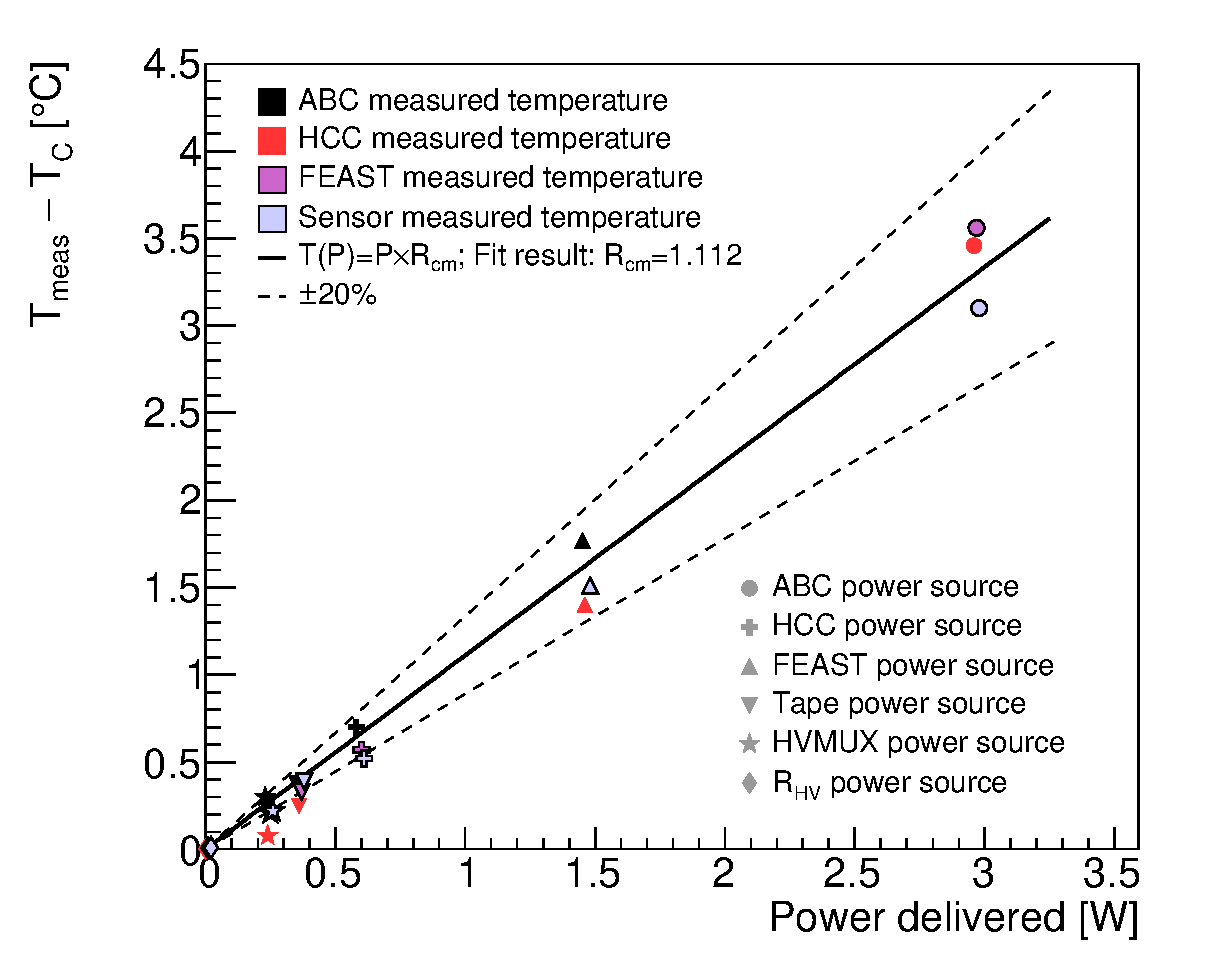
\includegraphics[width=0.49\linewidth]{figures/ThermalImpedanceFit_ShortStripEOS_Rcm.eps}}
\subfloat[] {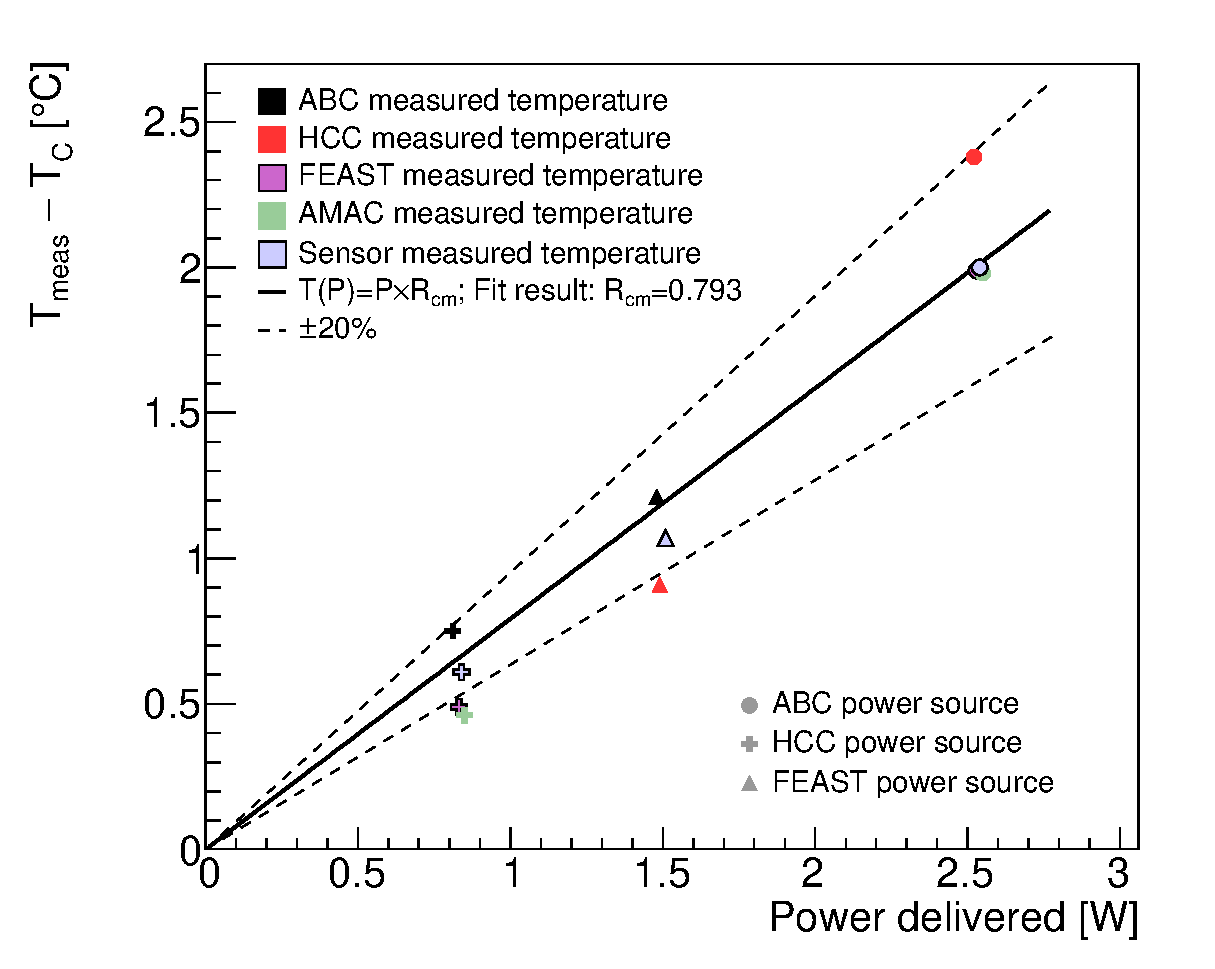
\includegraphics[width=0.49\linewidth]{figures/ThermalImpedanceFit_R0_Rcm.eps}}
\caption{The relationship between the power delivered to each front-end component and the temperature
of each component (as estimated by FEA). The slope of the fitted line is the estimate for $R_{CM}$.
(a) The fit for a short-strip barrel module. (b) The fit for the endcap R$_0$ module.
For each data point marker, the source of power is indicated by the shape, and the measured component is indicated
by the color.
In (b), the error bars represent the standard deviation of temperatures of
that particular component, and are not considered in the fit.
The blue band represents a $\pm$20\% error band on the fit for $R_{CM}$.
}
\label{fig:solving_for_Rcm}
\end{figure}

END ALTERNATE DESCRIPTION

For a barrel module this gives six sets of node temperatures for each source of injected heat. The thermal impedances in the network are then found from a fit of the linear network to this data. The agreement of the network temperatures using the thermal impedances from the fit with the data from FEA is better than 0.5$^\circ$C for all nodes. This procedure is performed for both, the EOS and the normal module. The thermal impedance from the sensor to the sink ($R_\text{M}+T_\text{C}$) in all cases is between 1.1 and 1.4~$^\circ$C/W, but higher values (between 10 and 20~$^\circ$C/W) are found for other impedances in the network ($R_\text{HCC}$ and $R_\text{FEAST}$), mostly because these are for components with a small footprint constituting a bottleneck for the heat flow.

\textit{[Georg has written the paragraph above to explain the fitting procedure – but is it confusingly different for the petals? I don’t know how he makes the fit].}

There are two recognised departures from linearity of the thermal path: the rise in thermal conductivity of the silicon sensor with decreasing temperature and the rise in heat transfer coefficient (HTC) to the evaporating CO$_2$ coolant with increasing thermal flux. The FEA models are run using mean values for these quantities appropriate to the operating conditions, and the thermoelectric model results are insensitive to the variations expected in practice.

\textit{[GAB: Should we expand on this with plots and tables? There are detailed differences between stave and petal that might be confusing, e.g. re coefficients for the sensor T.      Maybe all we could addin the end is confusion! ].}



